\documentclass[11pt,a4paper]{article}

\usepackage[margin=2.5cm]{geometry}
\usepackage{amsmath,amssymb,amsthm,mathtools}
\usepackage{graphicx}
\usepackage{booktabs}
\usepackage[dvipsnames]{xcolor}
\usepackage{enumitem}
\usepackage[colorlinks=true,linkcolor=MidnightBlue,citecolor=MidnightBlue,urlcolor=MidnightBlue]{hyperref}
\usepackage[capitalise,nameinlink]{cleveref}

% ---------------------------------------------------------------------------
% Drafting notes. Set \draftnotesfalse to hide every red note before submission.
\newif\ifdraftnotes \draftnotestrue
\newcommand{\note}[1]{\ifdraftnotes{\color{BrickRed}\textsf{\footnotesize[Draft note: #1]}}\fi}
% ---------------------------------------------------------------------------

\newtheorem{theorem}{Theorem}[section]
\newtheorem{proposition}[theorem]{Proposition}
\newtheorem{lemma}[theorem]{Lemma}
\newtheorem{corollary}[theorem]{Corollary}
\theoremstyle{definition}
\newtheorem{definition}[theorem]{Definition}
\newtheorem{question}{Question}
\theoremstyle{remark}
\newtheorem{remark}[theorem]{Remark}

\newcommand{\R}{\mathbb{R}}
\newcommand{\eps}{\varepsilon}
\newcommand{\Sph}{\mathbb{S}}
\newcommand{\Nb}{N^1_+\partial A}
\newcommand{\Lperp}{L_\perp}
\DeclareMathOperator{\spn}{span}
\DeclareMathOperator{\diag}{diag}

\title{\textbf{ESA: Boundaries of attractors with bounded noise:\\ boundary maps, normal hyperbolicity and singularities}\\[0.5em]
\large Early Stage Assessment report}
\author{John Parry\\[0.2em]
\small Department of Mathematics, Imperial College London\\
\small Supervisor(s): Professor Jeroen Lamb \quad Dynamical Systems group}
\date{\today}

\begin{document}
\maketitle
\begin{abstract}
    We look at bounded random dynamical systems - a class of dynamics which have spherical bounded noise injected at every iteration. Building on from the work of \note{Tei / Kourliouros - cite}, we look at a particular case of driving dynamics: linear contraction with quadratic resonance. We use this toy example to investigate the breakdown of normal hyperbolicity, and the resulting singularities which emerge as a result.  
\end{abstract}

\tableofcontents

%=============================================================================
\section{Introduction and problem statement}\label{sec:intro}
Real-world noise often comes in bounded form, for instance sensor accurate intervals, or rounding errors. When noise is bounded, trajectories can become trapped in a bounded invariant set. \note{These attractors support ergodic stationary measures that describe the system's statistics, and their bifurcations are topological: they occur when minimal invariant sets, which collide with, or detach from, other invariant objects. -> what does this mean? Ergodic stationary measure? system's statistics?} Understanding the \emph{shape} of these attractors is a prerequisite for a bifurcation theory of bounded-noise systems.  

\noindent We study iterations
\begin{equation}\label{eq:rds}
    x_{i+1} = f(x_i) + \xi_i,\qquad x_i\in\R^d, \qquad \xi_{i} \in \overline{B_{\epsilon}(0)}
\end{equation}
where $f$ is a diffeomorphism and the $\xi_i$ are i.i.d. random variables supported on the closed ball of radius
$\eps$. The \emph{compound} dynamics are captured by the set-valued map
\[
    F_{f,\eps}(C) = \overline{B_\eps(f(C))} = \{f(x)+y : x\in C,\ \|y\|\le\eps\},
\]
acting on $C \in \mathcal{K}(\R^n)$, the space of compact sets on $\R^n$. Attractors of~\eqref{eq:rds} - compact sets which are attracting and minimally forward invariant -
forward are fixed points of $F_{f,\eps}$; in the linear case the fixed point is unique and globally
attracting~\cite{LRT23,LRR15}.

\paragraph{The boundary map.}
The set-valued dynamics is lifted by the boundary map whose to the domain $\Nb=\{(x,n(x)): x\in\partial A\}\subset\R^d\times\Sph^{d-1}$ - the set of points with their outward unit normals. The boundary map is given by

\begin{equation}\label{eq:boundary-map}
  \beta_{f,\eps}(x,n) = \Bigl(f(x) + \eps\,\frac{Df(x)^{-T}n}{\|Df(x)^{-T}n\|},\ \frac{Df(x)^{-T}n}{\|Df(x)^{-T}n\|}\Bigr).
\end{equation}

 \note{Tei \& Kourliouros demonstrate that we can look at invariants of the boundary map and infer properties of the underlying set-valued system - ref.}

\note{Tei - ref} demonstrates the behaviour of the boundary map when our underlying dynamics is given by a linear contraction. \note{Talk about Kourliouros (ref) looking at the role of normal hyperbolciity, and how this manifests in linear paper.} 

\paragraph{The problem.}Let $f=L+\varphi$ where $L \in GL(\R^n)$ is the linear component, and $\varphi$ is of higher order, and regard $F_{f,\eps}$ as a perturbation of $F_{L,\eps}$. In a compact set, the linear map and its perturbation are $C^2$-close (in fact they are $C^\infty$ close). We will show that whilst we have a $C^2$-perturbation,  without normal hyperbolicity as hypothesised in \note{Kourliouros main theory}, the theorem fails to hold. We then investigate further the singularities which emerge as a result of this loss of normal hyperbolicity. The core problem is the converse situation:
\begin{quote}
\emph{When is normal hyperbolicity of the boundary map lost, and which singularities manifest as a result?} 
\end{quote}

In the plane, the first singularities expected on the boundary are wedges, that is, self-intersection points
($A_1$ in the terminology of the task sheet\footnote{In Arnold's notation a transverse double point of a front is the
multigerm $A_1^2$; $A_1$ alone denotes a regular point.}, cf.~\cite{Arn90}). The full front may additionally carry cusps ($A_2$). We will show that these emerge as artefacts of the front projection from the Legendrian submanifold. Concretely: 

\begin{enumerate}[label=\textbf{Task \arabic*.},leftmargin=*]
  \item For $L=\diag(\lambda_1,\lambda_2)$ with $0<\lambda_1<\lambda_2<1$ and $\lambda_2^2=\lambda_1$, show that
  $\beta_{L,\eps}$ is not normally hyperbolic at $\Nb$.
  \item At this resonance, show that there exist $C^2$-small perturbations $\varphi(x)=(ax_2^2,0)$, $a\neq0$, for which
  $\partial A'$ has singularities, and relate them to parameters $(a,\eps)$ for which $D\beta_{f,\eps}$ has complex eigenvalues.
  \item Determine the type, isolatedness and stability of these singularities, via the invariant Legendrian curve
  $\mathcal{L}'$ and its front.
\end{enumerate}


%=============================================================================
\section{Background and literature}\label{sec:background}

\subsection{Set-valued dynamics and minimal invariant sets}
Equip the space $\mathcal{K}(\R^d)$ of non-empty compact sets with the Hausdorff metric. Lamb, Rasmussen and
Rodrigues~\cite{LRR15} developed a topological bifurcation theory for minimal invariant sets of set-valued maps such as
$F_{f,\eps}$. In this theory, bifurcations are discontinuous changes of minimal invariant sets in the Hausdorff
metric, a phenomenon invisible to classical (deterministic or stochastic-differential) approaches. Zmarrou and
Homburg~\cite{ZH07} related such sets to bifurcations of stationary measures of random diffeomorphisms. Homburg and
Young~\cite{HY10} studied random differential equations with bounded noise on surfaces. For discrete-time linear
systems the attractor is a round ball when $L$ is a scalar multiple of an orthogonal matrix, and Lamb, Rasmussen and
Tey note, citing~\cite{HY10}, that solid ellipsoids essentially occur only in this conformal case~\cite{LRT23}.

A recurring difficulty is that minimal invariant sets of nonlinear systems may have complicated, non-smooth boundaries
and may coexist. Lamb, Rasmussen and Timperi~\cite{LRTi20a,LRTi20b} classified the singularities of boundaries of
$\eps$-neighbourhoods of planar sets, which is the local geometry generated by the ball $B_\eps$ in $F_{f,\eps}$. This
classification is the natural local model for the boundaries considered here.

\subsection{Linear maps with bounded noise}
For $f=L\in GL(d,\R)$, write $\mathcal{L}_\eps=F_{L,\eps}$. The following summarises~\cite{LRT23}.
\begin{theorem}[\cite{LRT23}]\label{thm:LRT}
$\mathcal{L}_\eps$ has a fixed point in $\mathcal{K}(\R^d)$ if and only if all eigenvalues of $L$ have modulus less
than~$1$. In that case:
\begin{enumerate}[label=(\roman*)]
  \item the fixed point $A=\lim_{k\to\infty}\mathcal{L}_\eps^k(\{0\})$ is unique and globally attracting, and is the
  unique attractor of~\eqref{eq:rds};
  \item $A$ is strictly convex, and $\partial A$ is $C^1$;
  \item $\Nb$ is globally attracting for $\beta_{L,\eps}$, and $\Nb=\{(x(n),n):n\in\Sph^{d-1}\}$ with
  \[ x(n)=\eps\sum_{k\ge0}L^k\Lperp^{-k}(n),\qquad \Lperp(n)=L^{-T}n/\|L^{-T}n\|;\]
  \item $\beta_{L,\eps}|_{\Nb}$ is topologically conjugate to $\Lperp$ on $\Sph^{d-1}$.
\end{enumerate}
\end{theorem}
Existence follows from the Banach fixed point theorem in an adapted norm. Convexity comes from the nested convex sets
$\mathcal{L}^k_\eps(0)$. Smoothness follows because every boundary point lies on the boundary of an $\eps$-ball contained in
$A$, so supporting hyperplanes are unique~\cite{Sch14}. Two questions are left open in~\cite{LRT23}: the \emph{precise}
smoothness of $\partial A$ (beyond $C^1$), and extensions to non-spherical noise. The paper also notes that $C^2$ smoothness is what is needed to apply the persistence theory of~\cite{KLRTTT23}. The
present project addresses the first question (\cref{sec:NH}) and then goes beyond the linear setting.

\subsection{The boundary map and its geometry}\label{sec:bm-geometry}
The boundary map~\eqref{eq:boundary-map} factorises as
\begin{equation}\label{eq:factorisation}
  \beta_{f,\eps} = \phi_\eps\circ P\circ h_f,\qquad
  \R^d\times\Sph^{d-1}\xrightarrow{\ h_f\ }\R^d\times(\R^d\setminus\{0\})\xrightarrow{\ P\ }\R^d\times\Sph^{d-1}
  \xrightarrow{\ \phi_\eps\ }\R^d\times\Sph^{d-1},
\end{equation}
with $h_f(x,n)=(f(x),Df(x)^{-T}n)$ (the dynamics), $P(x,n)=(x,n/\|n\|)$ (renormalisation) and
$\phi_\eps(x,n)=(x+\eps n,n)$ (the noise). Each factor has a geometric meaning, as follows.
\newline
\newline \noindent \emph{Normals transform by $Df^{-T}$.} A normal $n$ to a hypersurface $S$ at $x$ is characterised by what it
annihilates: $\langle n,u\rangle=0$ for all $u\in T_xS$. Pushing a curve $\gamma\subset S$ with $\gamma(0)=x$,
$\gamma'(0)=u$ forward gives $(f\circ\gamma)'(0)=Df(x)u\in T_{f(x)}f(S)$. So the new normal $n'$ must satisfy
$\langle n',Df(x)u\rangle=\langle Df(x)^Tn',u\rangle=0$ for all $u$, giving $n'\propto Df(x)^{-T}n$. Normals are
covectors, which explains the inverse transpose in~\eqref{eq:boundary-map}.
\newline
\newline\noindent\emph{The $\eps$-translation preserves normals.} If $\Gamma$ is a hypersurface with unit normal field $n$ and
$\Gamma_\eps=\{x+\eps n(x)\}$ is its outer equidistant, then differentiating $\Psi(x)=x+\eps n(x)$ along a curve gives
$D\Psi_x u=(I+\eps Dn_x)u$. Differentiating $\|n\|^2=1$ shows $Dn_xu\perp n(x)$, hence $T_{\Psi(x)}\Gamma_\eps=T_x\Gamma$, and
$n(x)$ is also the normal of $\Gamma_\eps$ at $\Psi(x)$. This justifies $\phi_\eps$.
\newline
\newline \emph{Renormalisation.} $D\pi_v=\frac{1}{\|v\|}\bigl(I-\frac{vv^T}{\|v\|^2}\bigr)=\frac{1}{\|v\|}\Pi_{v^\perp}$ for
$\pi(v)=v/\|v\|$. It kills the radial direction and scales the rest by $1/\|v\|$.

\begin{lemma}[conformal contact property]\label{lem:contact}
Let $\alpha=n\cdot dx$ on $\R^d\times\Sph^{d-1}$. Then
$\beta_{f,\eps}^*\alpha=\|Df(x)^{-T}n\|^{-1}\,\alpha$. In particular, $\beta_{f,\eps}$ is a contactomorphism, and
$\Nb$ is an invariant Legendrian submanifold whose front (projection $(x,n)\mapsto x$) is $\partial A$.
\end{lemma}
\begin{proof}
Write $\beta_{f,\eps}(x,n)=(f(x)+\eps n',n')$ with $n'=Df(x)^{-T}n/\|Df(x)^{-T}n\|$. Then
$\beta^*\alpha=n'\cdot(Df(x)\,dx+\eps\,dn')=(Df(x)^Tn')\cdot dx+\eps\,n'\cdot dn'$. Since $\|n'\|=1$, we have
$n'\cdot dn'=0$, and $Df(x)^Tn'=n/\|Df(x)^{-T}n\|$. On $\Nb$, $\alpha$ vanishes because $dx$ is tangent to
$\partial A$ and hence orthogonal to $n$.
\end{proof}

The contact property has a symplectic origin. Replace unit normals by unnormalised covectors (costates)
$p\in\R^d\setminus\{0\}$.

\subsection{Hyperbolicity, invariant manifolds and persistence}
A fixed point $p$ of a $C^1$ map $T$ is hyperbolic if $\sigma(DT(p))\cap\{|z|=1\}=\emptyset$. The stable and unstable
manifold theorem~\cite{KH95} then gives $C^1$ manifolds $W^{s,u}(p)$ with $T_pW^{s,u}=E^{s,u}$. More generally, a compact
invariant manifold $N$ is \emph{normally hyperbolic} (attracting) if there is a $DT$-invariant splitting
$T_N M = TN\oplus E^s$ with constants $C>0$ and $0<a<b$ such that, for all $k\ge0$,
\begin{equation}\label{eq:NH}
  \|DT^k|_{E^s}\|\le C a^k,\qquad m\bigl(DT^k|_{TN}\bigr)\ge C^{-1}b^k,
\end{equation}
where $m$ is the minimum norm. In words, normal contraction dominates tangential contraction. Fenichel~\cite{Fen71} and
Hirsch--Pugh--Shub~\cite{HPS77} proved that normally hyperbolic manifolds persist under $C^1$-small perturbations, with
smoothness controlled by the ratio of the rates ($r$-normal hyperbolicity: $a<b^r$ gives $C^r$ persistence). The
persistence paper~\cite{KLRTTT23} adapts this to boundary maps. Normal hyperbolicity of $\beta_{L,\eps}$ at $\Nb$ yields
$C^2$-persistence of attractor boundaries under nonlinear perturbations. Losing normal hyperbolicity is
therefore a natural (though not the only) route to singular boundaries.

\subsection{Legendrian fronts and their singularities}
Legendrian submanifolds of $(\R^d\times\Sph^{d-1},\alpha)$ project to \emph{fronts} in $\R^d$, which may be singular even
when the Legendrian is smooth~\cite{Arn90,AGV85,Gei08}. For planar fronts, the generic stable singularities are
transverse self-intersections ($A_1^2$, ``wedges'' when they lie on the boundary of a set) and semicubical cusps ($A_2$),
where the Legendrian curve becomes tangent to the fibre $\{x\}\times\Sph^1$. These are exactly the singularities that
appear on boundaries of $\eps$-neighbourhoods of planar sets~\cite{LRTi20a,LRTi20b}.

\subsection{Symplectic linear algebra and control: the two strands}
For a symplectic linear map, $\nu\in\sigma$ implies $1/\nu\in\sigma$, and eigenvalues on the unit circle can leave it
only through collisions of eigenvalues of opposite Krein signature~\cite{MS17}. For \emph{conformally} symplectic maps ($\omega\mapsto\rho\,\omega$), the
pairing becomes $\nu\leftrightarrow\rho/\nu$, and Wojtkowski and Liverani~\cite{WL98} showed the corresponding pairing of
Lyapunov exponents. Conformally symplectic systems model dissipative mechanics and admit a KAM theory~\cite{CCdlL13}. A
contactomorphism with $T^*\alpha=\rho\alpha$ acts conformally symplectically on the contact planes $\ker\alpha$ with
respect to $d\alpha$, which is the starting point of strand~(A).

On the control side, the link between bounded-noise systems and control theory is classical: minimal invariant sets
correspond to \emph{control sets}~\cite{CK00}, and the geometric theory of optimal control describes reachable-set
boundaries through Pontryagin extremals and their singularities~\cite{PBGM62,AS04}. \Cref{lem:pontryagin} identifies the
boundary map with these extremals, which is the starting point of strand~(B).

\subsection{Assessment and gaps}
The linear theory~\cite{LRT23} establishes existence, convexity and $C^1$ smoothness, and the persistence
theory~\cite{KLRTTT23} gives $C^2$-persistence under normal hyperbolicity. Missing are: (a) a characterisation of
\emph{when} $\beta_{L,\eps}$ is normally hyperbolic in terms of $\sigma(L)$, together with the exact regularity of
$\partial A$; (b) a description of what happens to $\partial A'$ when normal hyperbolicity fails; and (c) a connection
between the dynamics of $\beta_{f,\eps}$ (spectra at fixed points, invariant manifolds) and the singularity theory of
fronts. Question~(a) is answered for diagonal planar $L$ below. Questions~(b) and~(c) form the main thesis programme.

The resonant example of Task~2 deserves comment. For a contraction with eigenvalues $\lambda_1=\lambda_2^2$, the
monomial $x_2^2e_1$ is a \emph{resonant} term: by Poincar\'e--Sternberg theory~\cite{Ste57} it cannot be removed by a
smooth change of coordinates. The perturbation $\varphi=(ax_2^2,0)$ is therefore not a coordinate artefact. It is the
first genuinely nonlinear term compatible with the resonance.

%=============================================================================
\section{Preliminary results: the planar diagonal case}\label{sec:results}

Throughout this section $d=2$, $f=L=\diag(\lambda_1,\lambda_2)$ with $0<\lambda_1<\lambda_2<1$, and we write
\[
  \mu\coloneqq\frac{\lambda_1}{\lambda_2}\in(0,1),\qquad \beta\coloneqq\beta_{L,\eps},\qquad
  \beta(x,n)=\bigl(Lx+\eps\Lperp(n),\ \Lperp(n)\bigr),\quad \Lperp(n)=\frac{L^{-1}n}{\|L^{-1}n\|}.
\]
We use coordinates $(x_1,x_2,\theta)$ on $\R^2\times\Sph^1$ with $n=(\cos\theta,\sin\theta)$, and the frame
$\{\partial_{x_1},\partial_{x_2},\partial_\theta\}$, where $\partial_\theta$ corresponds to $(-\sin\theta,\cos\theta)$.

\subsection{Skew-product structure and fixed points}
For linear $f$ the normal component of $\beta$ does not depend on $x$:
\[
  \beta(x,n)=\bigl(\beta_1(x,n),\beta_2(n)\bigr),\qquad \beta_1(x,n)=Lx+\eps\beta_2(n),\qquad \beta_2=\Lperp .
\]
So $\beta$ is a \emph{skew product}: the normal dynamics on $\Sph^1$ are autonomous and drive the position dynamics.
This triangular structure is what makes the linear case solvable. It breaks for nonlinear $f$ because $Df(x)$, and
hence the normal update, then depends on $x$.

\begin{proposition}[fixed points]\label{prop:fixed}
$\beta$ has exactly four fixed points:
\[
  p_\pm=\Bigl(\bigl(\pm\tfrac{\eps}{1-\lambda_1},0\bigr),\ \pm e_1\Bigr),\qquad
  q_\pm=\Bigl(\bigl(0,\pm\tfrac{\eps}{1-\lambda_2}\bigr),\ \pm e_2\Bigr).
\]
\end{proposition}
\begin{proof}
$\beta(x,n)=(x,n)$ is equivalent to (II) $\Lperp(n)=n$ and (I) $Lx+\eps n=x$. Equation (II) says that
$L^{-1}n=\gamma n$ with $\gamma=\|L^{-1}n\|>0$, i.e.\ $n$ is a unit eigenvector of $L$ (eigenvalue $\gamma^{-1}>0$). Since
$\lambda_1\neq\lambda_2$, we have $\det(L-\gamma^{-1}I)=0$ only for $\gamma^{-1}\in\{\lambda_1,\lambda_2\}$, giving
$n\in\{\pm e_1,\pm e_2\}$. All four survive because both eigenvalues are positive. Then (I) gives
$x=\eps(I-L)^{-1}n$, which is well defined since $1\notin\sigma(L)$.
\end{proof}

The second equation has $d-1$ unknowns and is solved first; the first then determines $x$. This mirrors the triangular
structure. Geometrically, $p_\pm$ and $q_\pm$ are the points of $\partial A$ where the outward normal is an
eigenvector of $L$. Since $\frac{1}{1-\lambda_1}<\frac{1}{1-\lambda_2}$, the attractor is elongated along $e_2$, the
weakly contracting direction (\cref{fig:bm}(a)).

\subsection{Linearisation}
By the chain rule applied to~\eqref{eq:factorisation}, in ambient coordinates on $\R^2\times\R^2$ we get
\begin{equation}\label{eq:jacobian}
\begin{aligned}
  J_\beta(x,n)&=J_{\phi_\eps}J_PJ_{h_L}
  =\begin{pmatrix} I&\eps I\\0&I\end{pmatrix}\begin{pmatrix} I&0\\0&\tfrac{1}{\|v\|}\Pi_{v^\perp}\end{pmatrix}
   \begin{pmatrix} L&0\\0&L^{-T}\end{pmatrix}\\
  &=\begin{pmatrix} L&\eps\,D\Lperp\\0&D\Lperp\end{pmatrix},
  \qquad D\Lperp\coloneqq\tfrac{1}{\|v\|}\Pi_{v^\perp}L^{-T},
\end{aligned}
\end{equation}
with $v=L^{-T}n$. Two consequences follow.

\begin{lemma}\label{lem:triangular}
\begin{enumerate}[label=(\roman*)]
  \item $\sigma(J_\beta)=\sigma(L)\cup\sigma(D\Lperp)$, because the characteristic polynomial of a block
  upper-triangular matrix is the product of those of its diagonal blocks.
  \item The subspace $V=\R^2\oplus0$ of pure position displacements is invariant, with $J_\beta(w,0)=(Lw,0)$ at
  \emph{every} point. The ``old position'' has no influence on the ``new direction''.
\end{enumerate}
\end{lemma}

In~\eqref{eq:jacobian} the block $D\Lperp$ always has a zero eigenvalue in the radial direction. This is an artefact
of working in $\R^2\supset\Sph^1$, and restricting to $T\Sph^1=n^\perp$ removes it. Doing so gives a $3\times3$
Jacobian in the frame $\{\partial_{x_1},\partial_{x_2},\partial_\theta\}$. In angle coordinates the induced circle map
is
\begin{equation}\label{eq:circle}
  \tan\theta'=\mu\tan\theta,\qquad g'(\theta)\coloneqq\frac{d\theta'}{d\theta}=\frac{\mu}{\cos^2\theta+\mu^2\sin^2\theta}\in[\mu,\mu^{-1}].
\end{equation}

\begin{proposition}[spectra and eigenvectors]\label{prop:spectra}
In the frame $\{\partial_{x_1},\partial_{x_2},\partial_\theta\}$,
\[
  J_\beta(p_+)=\begin{pmatrix}\lambda_1&0&0\\0&\lambda_2&\eps\mu\\0&0&\mu\end{pmatrix},\qquad
  J_\beta(q_+)=\begin{pmatrix}\lambda_1&0&-\eps\mu^{-1}\\0&\lambda_2&0\\0&0&\mu^{-1}\end{pmatrix}.
\]
Hence $\sigma(J_\beta(p_\pm))=\{\lambda_1,\lambda_2,\mu\}\subset(0,1)$, so $p_\pm$ are sinks, and
$\sigma(J_\beta(q_\pm))=\{\lambda_1,\lambda_2,\mu^{-1}\}$, so $q_\pm$ are saddles with one-dimensional unstable manifolds.
The eigenvectors are given in \cref{tab:eig}, with
\[
  R=\frac{\eps\lambda_1}{\lambda_1-\lambda_2^2}\quad(\lambda_1\neq\lambda_2^2),\qquad
  \tilde R=\frac{\eps\lambda_2}{\lambda_2-\lambda_1^2}>0.
\]
\end{proposition}

\begin{table}[ht]
\centering
\small
\begin{tabular}{@{}lll@{\quad}lll@{}}
\toprule
\multicolumn{3}{c}{$p_+$ (sink)} & \multicolumn{3}{c}{$q_+$ (saddle)}\\
\cmidrule(r){1-3}\cmidrule(l){4-6}
eigenvalue & eigenvector & type & eigenvalue & eigenvector & type\\
\midrule
$\lambda_1$ & $\partial_{x_1}=(1,0,0)$ & normal & $\lambda_1$ & $\partial_{x_1}$ & normal\\
$\lambda_2$ & $\partial_{x_2}=(0,1,0)$ & normal & $\lambda_2$ & $\partial_{x_2}$ & normal\\
$\mu$ & $(0,R,1)$ & tangent$^{*}$ & $\mu^{-1}$ & $(-\tilde R,0,1)$ & tangent\\
\bottomrule
\end{tabular}
\caption{Spectral data at $p_+$ and $q_+$; ``tangent'' means tangent to $\Nb$ ($^{*}$when $\lambda_1>\lambda_2^2$, see \cref{sec:NH}). At $p_-$ and $q_-$ the eigenvalues coincide, and the $\theta$-eigenvectors are
$(0,-R,1)$ and $(\tilde R,0,1)$ (\cref{rem:symmetry}).}
\label{tab:eig}
\end{table}

\begin{proof}
At $p_+$, $\theta=0$ and $g'(0)=\mu$ by~\eqref{eq:circle}. Since $\partial_\theta n'=(-\sin\theta',\cos\theta')=e_2$
at $\theta'=0$, the $x$-component $Lx+\eps n'$ has $\theta$-derivative $\eps\mu e_2$. At $q_+$, $\theta=\pi/2$:
by~\eqref{eq:circle}, $g'(\pi/2)=\mu^{-1}$ and $\partial_\theta n'=-e_1$, which gives the matrices. For the
eigenvectors, at $p_+$ with eigenvalue $\mu$ we need $(\lambda_2-\mu)w_2+\eps\mu w_3=0$; taking $w_3=1$ gives
$w_2=\eps\mu/(\mu-\lambda_2)=R$. At $q_+$ with eigenvalue $\mu^{-1}$ we need $(\lambda_1-\mu^{-1})w_1-\eps\mu^{-1}=0$, so
$w_1=-\tilde R$. The remaining eigenvectors are immediate since $L$ is diagonal.
\end{proof}

\begin{remark}[the $\pm$ symmetry]\label{rem:symmetry}
The involution $\sigma(x,n)=(-x,-n)$ satisfies $\beta_{f,\eps}\circ\sigma=\sigma\circ\beta_{f,\eps}$ whenever $f$ is
odd, $f(-x)=-f(x)$: then $Df(-x)=Df(x)$ and $\beta_{f,\eps}(-x,-n)=-\beta_{f,\eps}(x,n)$. This is why $p_+\leftrightarrow p_-$
and $q_+\leftrightarrow q_-$ share spectra, with $D\sigma=\diag(-1,-1,1)$ mapping the eigenvectors as in
\cref{tab:eig}. The symmetry \emph{breaks} for the Task~2 map $f_a(x)=(\lambda^2x_1+ax_2^2,\lambda x_2)$, which is even in $x_2$.
Since $f_a(-x)=-f_{-a}(x)$, $\sigma$ instead conjugates $\beta_{f_a,\eps}$ to $\beta_{f_{-a},\eps}$, so the sides of $A'$
near $p_+$ and $p_-$ swap roles when $a$ changes sign. The reflection $(x_1,x_2,\theta)\mapsto(x_1,-x_2,-\theta)$ remains a
symmetry for every $a$, because $f_a$ commutes with $\diag(1,-1)$.
\end{remark}

\subsection{Global structure of the invariant normal bundle}

By~\eqref{eq:circle} the circle map $\Lperp$ has attracting fixed points $\theta\in\{0,\pi\}$ (derivative $\mu$) and
repelling fixed points $\theta=\pm\pi/2$ (derivative $\mu^{-1}$). Every other orbit moves monotonically from $\pm e_2$
towards $\pm e_1$.

\begin{proposition}\label{prop:structure}
$\Nb=\{p_+,p_-\}\cup W^u(q_+)\cup W^u(q_-)$. Each $W^u(q_\pm)$ consists of $q_\pm$ and two branches, which are
heteroclinic orbits to $p_+$ and $p_-$. In particular, the unstable set $\Sigma=\bigcup_{p\in\mathrm{Fix}(\beta)}W^u(p)$
equals $\Nb$, and all recurrent dynamics of $\beta|_{\Nb}$ is at the four fixed points.
\end{proposition}
\begin{proof}\note{[added] The notes pose the identity as a question (``what makes this true?''); this is a proof sketch using \cref{thm:LRT}.}
By \cref{thm:LRT}(iii),(iv), $\Nb$ is a compact invariant curve, the graph of $n\mapsto x(n)$ over $\Sph^1$, on which
$\beta$ is conjugate to $\Lperp$. Let $z=(x(n),n)\in\Nb$ with $n\notin\{\pm e_1\}$. Then $n$ lies in an open arc
bounded by some $\pm e_2$, and $\Lperp^{-k}(n)\to\pm e_2$, so $\beta^{-k}(z)\to q_\pm$ and $z\in W^u(q_\pm)$. Conversely,
$\Nb$ is a $\beta$-invariant curve through the saddle $q_\pm$ consisting near $q_\pm$ of points whose backward orbits stay
close to $q_\pm$, so it coincides locally with the one-dimensional local unstable manifold. Then
$W^u(q_\pm)=\bigcup_k\beta^k(W^u_{\mathrm{loc}})\subset\Nb$ by invariance. Finally, $p_\pm\notin W^u(q_\pm)$ because they are
fixed.
\end{proof}

This yields an algorithm for computing $\Nb$ (and later the Legendrian curve $\mathcal{L}'$ for nonlinear $f$, where no
series formula is available) by \emph{fundamental-domain iteration}. The steps are:
\begin{enumerate}
  \item Take the unstable eigenvalue $\kappa=\mu^{-1}$ and eigenvector $v^u$ of $J_\beta(q)$.
  \item Seed $N$ points on the fundamental domain $\{q+tv^u: t\in[\delta/\kappa,\delta]\}$ with $\delta\approx10^{-7}$. This
  segment is $O(\delta^2)$-close to $W^u(q)$ because $T_qW^u=E^u$.
  \item Iterate under $\beta$. The images $\beta^k(S)$ tile $W^u(q)$, and the initial error is contracted transversally
  (rates $\lambda_1,\lambda_2$) while the arc grows (rate $\kappa$).
\end{enumerate}

\subsection{Normal hyperbolicity and the resonance $\lambda_1=\lambda_2^2$ (Task 1)}\label{sec:NH}
\note{[added] The ingredients (spectra, $R$, the invariant subspace $V$) are all in the notes. The interpretation below was worked out while drafting, so check it carefully.}

Which direction is tangent to $\Nb$ at the sink $p_+$? Orbits approach $p_+$ along the weakest contracting direction
(\cref{rem:dynreading}). If $\lambda_1>\lambda_2^2$ then $\mu>\lambda_2$, so $\Nb$ is a $C^1$ graph over $\Sph^1$ with
$T_{p_+}\Nb=\spn\{(0,R,1)\}$ (tangential rate $\mu$), and the normal directions $\partial_{x_1},\partial_{x_2}$ contract at
rates $\lambda_1,\lambda_2$. If $\lambda_1<\lambda_2^2$ then $T_{p_+}\Nb=\spn\{\partial_{x_2}\}$ (tangential rate $\lambda_2$), because
$x'(\theta)\to\infty$ (\cref{prop:curvature}). At the resonance $\lambda_1=\lambda_2^2$ the eigenvector $(0,R,1)$
\emph{degenerates}: $\mu=\lambda_2$ is a double eigenvalue, $J_\beta(p_+)$ has a $2\times2$ Jordan block (confirmed numerically),
and again $T_{p_+}\Nb=\spn\{\partial_{x_2}\}$.

\begin{proposition}\label{prop:NH}
\begin{enumerate}[label=(\roman*)]
  \item At the resonance $\lambda_1=\lambda_2^2$, $\Nb$ admits no $D\beta$-invariant complement at $p_+$. Hence $\beta_{L,\eps}$ is
  not normally hyperbolic at $\Nb$ in any sense. \emph{(Task~1.)}
  \item With normal hyperbolicity in the uniform-rate form~\eqref{eq:NH}, $\beta_{L,\eps}$ is normally hyperbolic at $\Nb$ if
  and only if $\lambda_1>\lambda_2^2$.
\end{enumerate}
\end{proposition}
\begin{proof}[Proof sketch]
(i) $J_\beta(p_+)=\lambda_1\oplus J_2(\lambda_2)$, with a Jordan block on $\spn\{\partial_{x_2},\partial_\theta\}$. Its invariant
2-planes are $\spn\{\partial_{x_1},\partial_{x_2}\}$ and $\spn\{\partial_{x_2},\partial_\theta\}$, and both contain
$T_{p_+}\Nb=\spn\{\partial_{x_2}\}$.

(ii) \emph{Sufficiency.} Take $E^s=V=\R^2\oplus0$. By \cref{lem:triangular}(ii) it is invariant along all of $\Nb$, with
$D\beta^k|_{E^s}=L^k$, so $\|D\beta^k|_{E^s}\|=\lambda_2^k$. It is complementary to $T\Nb$ because $\Nb$ is a $C^1$ graph over
$\Sph^1$: the derivative series for $x'(\theta)$ converges uniformly when $\lambda_1>\lambda_2^2$. The $\theta$-coordinate
then gives a norm on $T\Nb$ uniformly equivalent to the ambient one, and in it
$m(D\beta^k|_{T\Nb})\ge\prod_j g'(\theta_j)\ge\mu^k$ by~\eqref{eq:circle}. So~\eqref{eq:NH} holds with $a=\lambda_2<b=\mu$.
\emph{Necessity.} Let $\lambda_1\le\lambda_2^2$. At the saddle $q_+$ the eigenvalues $\lambda_1,\lambda_2,\mu^{-1}$ are distinct
and $T_{q_+}\Nb=E^u$, so the only invariant complement is $V$. On $V$, $\|D\beta^k\|=\lambda_2^k$, which forces $a\ge\lambda_2$.
At $p_+$, $T_{p_+}\Nb=\spn\{\partial_{x_2}\}$ is contracted at rate $\lambda_2$, which forces $b\le\lambda_2$. Hence no constants
$a<b$ exist.
\end{proof}

\begin{remark}
The necessity argument is \emph{global}: it compares the normal rate at $q_\pm$ with the tangential rate at $p_\pm$. For
$\lambda_1<\lambda_2^2$ the \emph{local} domination condition at $p_+$ holds again (normal rates $\lambda_1,\mu$ versus
tangential $\lambda_2$). Numerical checks along the heteroclinic orbit $q_+\to p_+$ suggest that, under the relative
(pointwise) definition of Hirsch--Pugh--Shub~\cite{HPS77}, normal hyperbolicity may in fact hold in this regime, with a
splitting that rotates from $V$ at $q_+$ to $\spn\{\partial_{x_1},(0,R,1)\}$ at $p_+$. Only the resonance fails under every
definition.
\end{remark}
\note{Check which definition the persistence paper~\cite{KLRTTT23} uses. The referee check suggests it uses global constants, which matches~\eqref{eq:NH} and (ii).}

The geometric meaning is the curvature of $\partial A$ at its flattest points. Parametrise $\partial A$ by the normal
angle, $\theta\mapsto x(\theta)=x(n(\theta))$. Then $x'(\theta)$ is tangent to $\partial A$, and $|x'(\theta)|$ is the
radius of curvature. When $\Nb$ is a $C^1$ graph, its tangent vector $(x'(\theta),1)$ at a fixed point is the
$\theta$-eigenvector. So \emph{$\tilde R$ is the radius of curvature of $\partial A$ at $q_\pm$, and, when
$\lambda_1>\lambda_2^2$, $R$ is the radius of curvature at $p_\pm$.} (For $\lambda_1<\lambda_2^2$ we have $R<0$, and $(0,R,1)$ is
a strong-stable direction transverse to $\Nb$.)

\begin{proposition}[curvature at $p_\pm$ and $q_\pm$]\label{prop:curvature}
The curvature of $\partial A$ at $q_\pm$ is $(\lambda_2-\lambda_1^2)/(\eps\lambda_2)>0$. At $p_\pm$:
\begin{enumerate}[label=(\roman*)]
  \item if $\lambda_1>\lambda_2^2$, the curvature is $\kappa(p_\pm)=\dfrac{\lambda_1-\lambda_2^2}{\eps\lambda_1}>0$;
  \item if $\lambda_1\le\lambda_2^2$, the radius of curvature diverges as $\theta\to0$ and $\kappa(p_\pm)=0$. Numerically, the
  divergence is logarithmic, $|x'(\theta)|\sim\frac{\eps\log(1/|\theta|)}{\log(\lambda_2/\lambda_1)}$, at the resonance, and a
  power law $|x'(\theta)|\asymp|\theta|^{-\alpha}$ with $\alpha=\log(\lambda_2^2/\lambda_1)/\log(\lambda_2/\lambda_1)\in(0,1)$ when
  $\lambda_1<\lambda_2^2$.
\end{enumerate}
\end{proposition}
\begin{proof}[Proof of (i) and divergence in (ii)]
Since $L$ is symmetric, $\Lperp^{-k}(n)=L^kn/\|L^kn\|$, so by \cref{thm:LRT}(iii)
\[
  x_2(\theta)=\eps\sum_{k\ge0}\frac{\lambda_2^{2k}\sin\theta}{\sqrt{\lambda_1^{2k}\cos^2\theta+\lambda_2^{2k}\sin^2\theta}} .
\]
Differentiating termwise at $\theta=0$ gives $x_2'(0)=\eps\sum_k(\lambda_2^2/\lambda_1)^k$, which equals
$\eps\lambda_1/(\lambda_1-\lambda_2^2)=R$ if $\lambda_2^2<\lambda_1$ (uniform convergence of the derivative series near $\theta=0$).
Otherwise $x_2'(\theta)\to\infty$ as $\theta\to0$ by Fatou's lemma, since the terms are positive. Also $x_1'(0)=0$ by symmetry. The computation at $q_\pm$ is identical with the roles of the indices exchanged, and it always
converges since $\lambda_1^2<\lambda_2$. The asymptotic rates in (ii) follow heuristically by counting the terms with
$\mu^{-k}|\theta|\lesssim1$ and are confirmed numerically in \cref{fig:curv}.
\end{proof}

Some checks and consequences:
\begin{itemize}
  \item For $\lambda_1=\lambda_2=\lambda$ the formulas reduce to $\kappa=(1-\lambda)/\eps$, the curvature of the disc
  $A=B_{\eps/(1-\lambda)}(0)$.
  \item In all regimes the curvature $1/|x'(\theta)|$ is continuous, tending to $0$ at $p_\pm$ when $\lambda_1\le\lambda_2^2$. So
  $\partial A$ is $C^2$ in the diagonal planar case. This is consistent with the task sheet's statement that $\partial A$ is
  $C^2$, which goes beyond the $C^1$ proved in~\cite{LRT23}.
  \item Higher regularity is subtler. At the resonance the curvature has no H\"older modulus at $p_\pm$. For $\lambda_1>\lambda_2^2$,
  numerically $(R-|x'(\theta)|)/R\asymp|\theta|^{\gamma}$ with $\gamma=\log(\lambda_1/\lambda_2^2)/\log(\lambda_2/\lambda_1)$. Note that
  $\gamma<1$ exactly when $\lambda_1^2<\lambda_2^3$, i.e.\ when the $2$-normal hyperbolicity condition $\lambda_2<\mu^2$ fails at
  $p_\pm$. This links $r$-normal hyperbolicity to the precise smoothness question left open in~\cite{LRT23}.
\end{itemize}
\note{The ``not better than'' statements are conjectures from the asymptotics. They need proofs, and are natural first lemmas for the thesis.}

\begin{remark}[a dynamical reading]\label{rem:dynreading}
At $p_+$, orbits approach along the \emph{weakest} contracting direction. If $\lambda_1>\lambda_2^2$ this is the
tangential direction ($\mu>\lambda_2$), so $\Nb$ is a smooth graph and $\partial A$ is genuinely curved at $p_\pm$. If
$\lambda_1<\lambda_2^2$ the weakest direction is $\partial_{x_2}$, which is normal to the fibre, so $\Nb$ arrives at $p_+$
tangent to $\partial_{x_2}$. In that case $\theta\sim|x_2|^{1/(1-\alpha)}$ along $\Nb$, and $\partial A$ is flat to higher
order at $p_\pm$. The resonance is the transition between the two regimes, which is where the task sheet expects
singularities to be born under the perturbation $\varphi$.
\end{remark}

\subsection{Contact spectral pairing: a linear contact algebra viewpoint}\label{sec:pairing}
\note{[added] Strand (A) in action. The general statement is standard reasoning but should be checked against the literature on conformally symplectic linear algebra.}

\begin{proposition}[spectral pairing at fixed points]\label{prop:pairing}
Let $T$ be a contactomorphism of a $(2m+1)$-manifold with $T^*\alpha=\rho\,\alpha$, and let $T(z)=z$. Then $DT_z$
preserves $\xi_z=\ker\alpha_z$, acts on $T_zM/\xi_z$ as multiplication by $\rho(z)$, and $DT_z|_{\xi_z}$ is conformally
symplectic for $d\alpha|_{\xi_z}$ with factor $\rho(z)$. Hence
\[
  \sigma(DT_z)=\{\rho(z)\}\ \cup\ \{\nu_1,\rho/\nu_1,\dots,\nu_m,\rho/\nu_m\}.
\]
\end{proposition}
\begin{proof}
At a fixed point, $\alpha_z(DT_zv)=\rho(z)\alpha_z(v)$, which gives the first two claims. Moreover
$T^*d\alpha=d\rho\wedge\alpha+\rho\,d\alpha$, and on $\xi_z$ the first term vanishes. A linear map $S$ with
$S^*\omega=\rho\,\omega$ satisfies $S^T\Omega S=\rho\,\Omega$, so $S$ is similar to $\rho S^{-T}$ and its spectrum is invariant under
$\nu\mapsto\rho/\nu$.
\end{proof}

For the boundary map, $\rho=\|Df(x)^{-T}n\|^{-1}$ (\cref{lem:contact}). In the diagonal case, $\xi_{p_+}=\spn\{\partial_{x_2},\partial_\theta\}$
and $\rho(p_+)=\|L^{-1}e_1\|^{-1}=\lambda_1$. Indeed $\sigma(J_\beta(p_+))=\{\lambda_1\}\cup\{\lambda_2,\lambda_1/\lambda_2\}$, and
the pair multiplies to $\rho$. At $q_\pm$, $\rho=\lambda_2$ and the pair is $\{\lambda_1,\lambda_2/\lambda_1\}$. This
reorganises \cref{sec:NH}:
\begin{itemize}
  \item The Legendrian tangent direction lies in $\xi$ (Legendrian submanifolds are tangent to $\ker\alpha$), so it carries
  one member $\nu_T$ of a pair. Since orbits approach a sink along the weakest direction, $\nu_T$ is the \emph{larger}
  member of the pair: $\nu_T=\mu$ if $\lambda_1>\lambda_2^2$ and $\nu_T=\lambda_2$ if $\lambda_1<\lambda_2^2$.
  \item The resonance $\lambda_1=\lambda_2^2$ is precisely the \emph{collision} $\nu=\rho/\nu=\sqrt\rho$ within the pair, where
  the Legendrian tangent switches from one member of the pair to the other. Locally at $p_\pm$ this collision is the only
  place where normal hyperbolicity fails (\cref{prop:NH}(i)). The failure on the whole region $\lambda_1<\lambda_2^2$ under
  the uniform definition (\cref{prop:NH}(ii)) is a global mismatch between $p_\pm$ and $q_\pm$.
  \item By analogy with Krein collisions, a generic perturbation through a collision can send the pair into the complex
  plane, onto the circle $|\nu|=\sqrt{\rho}$. This is the mechanism suggested by the task sheet for the birth of
  singularities. We verified the pairing numerically at fixed points of boundary maps of a non-diagonal linear map,
  the Task~2 map and a H\'enon-like map. In each case the eigenvalues on $\xi$ multiply to $\rho$ to machine precision.
\end{itemize}

\subsection{Numerical experiments}\label{sec:numerics}
\note{[added] Figures and checks generated while drafting with the attached \texttt{boundary\_map\_numerics.py} and \texttt{pairing\_checks.py} (JAX). Re-run and adapt them yourself.}
The boundary map was implemented in \textsc{JAX} in the coordinates $(x_1,x_2,\theta)$, with Jacobians computed by automatic
differentiation. The following checks were performed:
\begin{itemize}
  \item the fixed points of \cref{prop:fixed} satisfy $|\beta(z)-z|<10^{-15}$, and the spectra and eigenvectors of
  \cref{prop:spectra} are reproduced to machine precision for $(\lambda_1,\lambda_2)=(0.3,0.5)$ and $(0.4,0.7)$, including the
  sign of $(-\tilde R,0,1)$ at $q_+$;
  \item $W^u(q_\pm)$ from fundamental-domain iteration agrees with the series of \cref{thm:LRT}(iii) to $3\times10^{-15}$,
  confirming \cref{prop:structure} (\cref{fig:bm});
  \item $\beta^*\alpha=\alpha/\|L^{-T}n\|$ at random points (\cref{lem:contact});
  \item at $(\lambda_1,\lambda_2)=(0.49,0.7)$, $J_\beta(p_+)$ has $\operatorname{rank}(J_\beta-\lambda_2I)=2$, i.e.\ a Jordan block;
  \item the radius of curvature at $p_+$ converges to $R$ as $\theta\to0$ in the normally hyperbolic regime (at $\theta=10^{-10}$ it is
  $5.998$ versus $R=6$, with the correction $\asymp\theta^\gamma$), has fitted log-slope $-1.4427$
  (predicted $-1/\log2$) at the resonance $(0.25,0.5)$, and has fitted power $-0.247$ (predicted $-0.2435$) at $(0.2,0.5)$
  (\cref{fig:curv}).
\end{itemize}

\begin{figure}[ht]
\centering
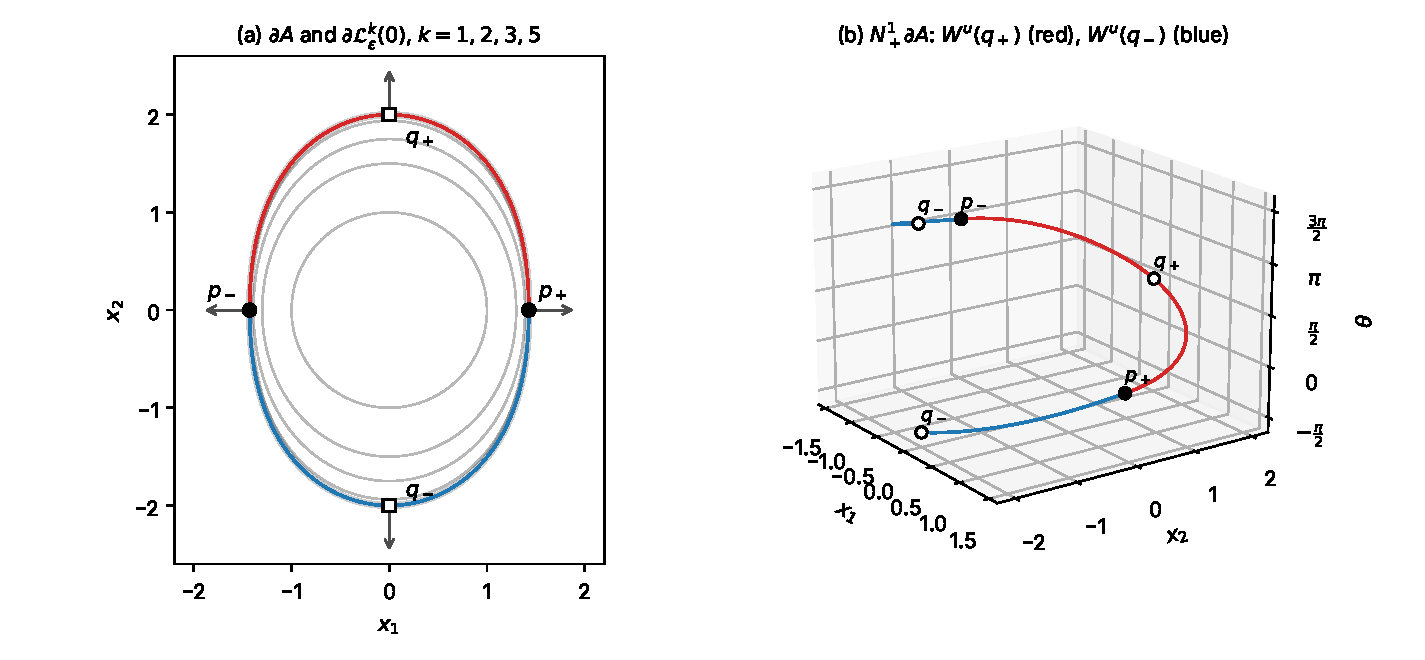
\includegraphics[width=\textwidth]{fig_boundary_map.pdf}
\caption{$(\lambda_1,\lambda_2,\eps)=(0.3,0.5,1)$. (a) The attractor boundary $\partial A$ (thick grey), with the nested
sets $\partial\mathcal{L}^k_\eps(0)$ converging to it, and the projections of $W^u(q_+)$ (red) and $W^u(q_-)$ (blue)
computed by fundamental-domain iteration. Arrows are the outward normals at the fixed points. (b) The same curves in
$\R^2\times\Sph^1$: the Legendrian curve $\Nb$ is the union of the four fixed points and the four heteroclinic branches.}
\label{fig:bm}
\end{figure}

\begin{figure}[ht]
\centering
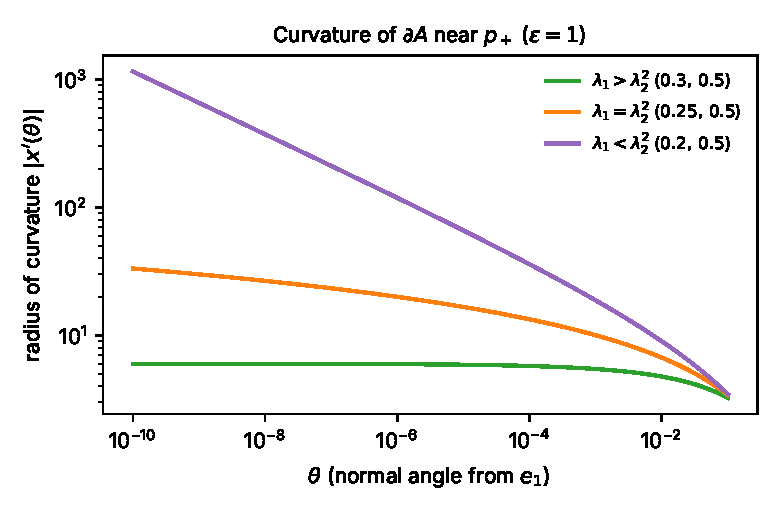
\includegraphics[width=0.62\textwidth]{fig_curvature.pdf}
\caption{Radius of curvature $|x'(\theta)|$ of $\partial A$ near $p_+$ in the three regimes of \cref{prop:curvature}:
bounded (normally hyperbolic), logarithmic divergence (resonance), power-law divergence.}
\label{fig:curv}
\end{figure}

%=============================================================================
\section{Research plan}\label{sec:plan}

\subsection{Next steps: the resonant perturbation (Tasks 2 and 3)}\label{sec:plan-tasks}
Fix $\lambda_1=\lambda^2$, $\lambda_2=\lambda$ and $f(x)=(\lambda^2x_1+ax_2^2,\ \lambda x_2)$. This is a diffeomorphism with
$f^{-1}(y)=(\lambda^{-2}(y_1-a\lambda^{-2}y_2^2),\lambda^{-1}y_2)$ and $Df(0)=L$.

\begin{enumerate}[label=\textbf{(\alph*)},leftmargin=*]
  \item \textbf{Fixed points of $\beta_{f,\eps}$.} These solve $x-f(x)=\eps n$ and $Df(x)^Tn=cn$ with $c>0$, where
  \[
    Df(x)^{-T}=\begin{pmatrix}\lambda^{-2}&0\\-2ax_2\lambda^{-3}&\lambda^{-1}\end{pmatrix}.
  \]
  \note{The notes use $(L+\varphi)^{-T}=L^{-T}+\varphi^{-T}$, which does not hold. The boundary map needs the derivative $Df(x)^{-T}=(L+D\varphi(x))^{-T}$, as above.}
  Since $Df(x)^T$ is lower triangular with diagonal $(\lambda^2,\lambda)$, either $n=\pm e_2$ ($c=\lambda$; continuations of $q_\pm$,
  with $x=(a x_2^2/(1-\lambda^2),\pm\eps/(1-\lambda))$), or $c=\lambda^2$ and $n_2=2ax_2n_1/(\lambda^2-\lambda)$. Combined with
  $x_2=\eps n_2/(1-\lambda)$, the latter gives $n_2=0$ ($p_\pm$, unchanged) or
  \[
    n_1=-\frac{\lambda(1-\lambda)^2}{2a\eps},\qquad n_2=\pm\sqrt{1-n_1^2},\qquad x_2=\frac{\eps n_2}{1-\lambda},\quad
    x_1=\frac{\eps n_1+ax_2^2}{1-\lambda^2}.
  \]
  \note{[added] Derived while drafting and checked numerically (residual $\sim10^{-17}$).}
  This pair of extra fixed points exists iff $|a|\eps>\lambda(1-\lambda)^2/2$, and it is related by the reflection of
  \cref{rem:symmetry}. Numerically they are sinks; at $\lambda=0.6$, $\eps=0.5$, $a=0.2$ their spectrum is
  $\{0.36,0.768,0.469\}$, and the pair in $\xi$ again multiplies to $\rho$. Note also that the isotropic rescaling
  $x\mapsto cx$ sends $(a,\eps)\mapsto(a/c,c\eps)$, so for fixed $\lambda$ the problem depends only on the product $a\eps$. The
  bifurcation study is therefore one-parameter, in $a\eps$, and every threshold below is a condition on $a\eps$.
  \item \textbf{Spectra.} The Jacobian is no longer block-triangular (\cref{lem:triangular} fails because the normal
  update depends on $x$). Compute $\sigma(D\beta_{f,\eps})$ at the fixed points and locate the curves in the
  parameter $a\eps$ where eigenvalues become complex. The task sheet's hint links these to the birth of singularities.
  A first computation is encouraging.\note{[added] Two-line computation plus numerical check; verify.} The points $p_\pm$
  survive unchanged, since $f(x_1,0)=(\lambda^2x_1,0)$, and $\rho(p_\pm)=\lambda^2$. On $\xi_{p_+}=\spn\{\partial_{x_2},\partial_\theta\}$,
  however, the nonlinearity creates the coupling $\partial\theta'/\partial x_2=-2a/\lambda$, giving
  \[
    D\beta_{f,\eps}(p_+)|_{\xi}=\begin{pmatrix}\lambda-2a\eps/\lambda & \eps\lambda\\ -2a/\lambda & \lambda\end{pmatrix},
    \qquad \det=\lambda^2=\rho,\quad \operatorname{tr}=2\lambda-\frac{2a\eps}{\lambda}.
  \]
  So the pair at $p_+$ is complex, on the circle $|\nu|=\lambda=\sqrt\rho$, if and only if $0<a\eps<2\lambda^2$. At $p_-$ the
  sign of $a$ flips, giving complex eigenvalues iff $-2\lambda^2<a\eps<0$. This is consistent with \cref{prop:pairing,rem:symmetry}, and
  numerically ($\lambda=0.6$, $a=0.4$, $\eps=0.5$) the eigenvalues at $p_+$ are $0.267\pm0.537i$.

  On the opposite side, the pair at $p_-$ is real for $a>0$, with trace $2\lambda+2a\eps/\lambda$. Its larger member exceeds
  $1$ iff $\operatorname{tr}>1+\rho$, i.e.\ iff $a\eps>\lambda(1-\lambda)^2/2$. This is \emph{the same threshold} at which the
  extra fixed points of~(a) appear, with $n_1\to-1$ as $a\eps\downarrow\lambda(1-\lambda)^2/2$. This strongly suggests a pitchfork
  bifurcation at $p_-$ (reflection-symmetric, hence a pitchfork) that turns $p_-$ into a saddle and creates the two new
  sinks. Numerically, at $\lambda=0.6$, $\eps=0.5$, $a=0.2$ the spectrum at $p_-$ is $\{0.36,1.244,0.289\}$.
  It is a natural candidate for singularities born while the eigenvalues are still \emph{real}, which is the task sheet's
  second question. The next steps are to relate the focus at $p_+$ and the saddle at $p_-$ to the geometry of
  $\mathcal{L}'$ near these points.
  \item \textbf{The invariant Legendrian curve $\mathcal{L}'$.} Construct it numerically as a union of unstable
  manifolds of saddles of $\beta_{f,\eps}$, using fundamental-domain iteration, and theoretically by a graph transform
  over $\Nb$. Show that $\mathcal{L}'\supseteq\overline{N^1_+\partial A'}$.
  \item \textbf{Fronts and singularities.} Project $\mathcal{L}'$ to the big front $\Gamma'\subset\R^2$. Detect
  self-intersections ($A_1^2$), and cusps ($A_2$, where $\mathcal{L}'$ is tangent to the fibre $\partial_\theta$, i.e.\
  $x'(\theta)=0$). Show that $\partial A'$ carries only wedges while $\Gamma'$ also has cusps in the interior of $A'$.
  Test the conjecture on the task sheet: the singularities are stable but not isolated, accumulating at the projection
  of a fixed point with complex eigenvalues. A focus-type fixed point would make $\mathcal{L}'$ spiral, producing
  infinitely many cusps.
  \item \textbf{Asymmetry.} Following \cref{rem:symmetry}, compare the two sides of $A'$ for $a>0$ and $a<0$.
\end{enumerate}

\subsection{Two broader strands}\label{sec:strands}
The task sheet is one instance of two more general programmes, which could form the second half of the thesis.

\paragraph{(A) Linear contact algebra.} Linear symplectic algebra (the group $Sp(2m)$, its spectral symmetry, normal
forms of symplectic matrices, Krein signature and collisions~\cite{MS17}) underpins Hamiltonian dynamics. The analogous
\emph{linear contact algebra} concerns the linearisations $DT_z$ of contactomorphisms at fixed and periodic points,
equivalently the group of linear maps of $(\R^{2m+1},\alpha)$ preserving $\ker\alpha$ conformally with induced
conformally symplectic action. Questions:
\begin{enumerate}[label=(A\arabic*),leftmargin=*]
  \item Normal forms of linear contactomorphisms under linear contact conjugacy. Which Jordan structures are allowed,
  and what is the analogue of Krein signature for colliding pairs $\nu=\rho/\nu$?
  \item Which spectral configurations are realised by boundary maps? Here $\rho=\|Df^{-T}n\|^{-1}$ is tied to $f$, which
  may constrain e.g.\ $\rho$ relative to the pair. Classify the codimension-one degenerations (collisions, $|\nu|=1$,
  $\nu=\rho$) and match each with a regularity or singularity phenomenon of attractor boundaries. \Cref{prop:NH,prop:pairing}
  give the first entry of such a dictionary: pair collision at a sink $\Leftrightarrow$ switch of the Legendrian tangent
  between the members of the pair $\Leftrightarrow$ transition from positive to vanishing curvature of $\partial A$ at
  $p_\pm$, and local failure of normal hyperbolicity.
  \item Lyapunov-exponent pairing along $\Nb$~\cite{WL98} and its consequences for $C^r$ regularity of $\partial A$ via
  $r$-normal hyperbolicity.
  \item Higher dimensions: several pairs, and resonances between them.
\end{enumerate}

\paragraph{(B) Pontryagin flows and control theory.} By \cref{lem:pontryagin}, boundary maps are spherised
Pontryagin extremal maps, and in continuous time the boundary dynamics is the contact reduction of the Pontryagin
flow of $H=\langle p,F(x)\rangle+\eps\|p\|$. Questions:
\begin{enumerate}[label=(B\arabic*),leftmargin=*]
  \item Make the dictionary precise: attractors and minimal invariant sets $\leftrightarrow$ (closures of) reachable sets
  and control sets~\cite{CK00}; boundaries $\leftrightarrow$ envelopes of extremals; invariant Legendrian submanifolds
  $\leftrightarrow$ invariant Lagrangian cones of the Pontryagin Hamiltonian system.
  \item Import results: singularities of reachable sets and optimal syntheses (switching curves, conjugate points,
  cut loci)~\cite{AS04} should correspond to wedges and cusps of fronts. In particular, cusps of the big front
  $\Gamma'$ should be conjugate-point (caustic) phenomena of the extremal flow. This would give a control-theoretic
  route to Task~3.
  \item Continuous time: attractors of random differential equations with bounded noise~\cite{HY10} via the
  Pontryagin flow, with the boundary map recovered as a time-$h$ map.
  \item Numerics: exploit the extremal formulation (shooting, continuation of extremals) in JAX, alongside the
  fundamental-domain methods of \cref{sec:results}.
  \item Beyond spherical noise: for a general convex control set $U$, $\eps\|p\|$ becomes the support function $h_U(p)$,
  which handles the non-spherical noise question of~\cite{LRT23} within the same framework.
\end{enumerate}

\subsection{Longer-term directions}
\begin{enumerate}[leftmargin=*]
  \item \textbf{Regularity of $\partial A$ for general linear $L$.} Extend \cref{prop:NH,prop:curvature} to $d\ge2$ and to
  non-diagonalisable $L$ or $L$ with complex eigenvalues. In the latter case $\Lperp$ has no fixed points on $\Sph^1$, and the
  dynamics on $\Nb$ is a circle rotation. Relate $r$-normal hyperbolicity ($a<b^r$) to $C^r$ regularity of $\partial A$.
  \item \textbf{Persistence and bifurcation of boundaries.} Combine the singularity picture with the persistence
  theory~\cite{KLRTTT23} to describe codimension-one bifurcations of attractor boundaries. Connect this with the planar
  classification of~\cite{LRTi20a,LRTi20b}.
  \item \textbf{Nonlinear examples and numerics.} Apply the methods to genuinely nonlinear systems, e.g.\ the H\'enon map
  with bounded noise~\cite{LRT25}. Build a reusable JAX toolbox for boundary maps (automatic Jacobians, invariant-manifold
  continuation), and compare with $\eps$-chain and set-oriented methods.
\end{enumerate}

\subsection{Timeline to the Late Stage Review}
\note{Adjust months to your actual start date; the LSR is due by month 24.}
\begin{center}
\small
\begin{tabular}{@{}lp{0.78\textwidth}@{}}
\toprule
Period & Goal\\
\midrule
Months 12--14 & Task 2(a,b): fixed points and spectra of $\beta_{f,\eps}$; numerical bifurcation diagram in $a\eps$.\\
Months 14--17 & Task 2(c,d): Legendrian curve and front; numerical evidence of wedges and cusps.\\
Months 17--20 & Task 3: classification and stability of the singularities; proofs in the simplest cases.\\
Months 20--22 & Rigorous version of \cref{prop:NH,prop:curvature,prop:pairing} for general planar $L$; draft paper.\\
Throughout & Reading for strands (A) and (B): linear symplectic algebra and Krein theory; geometric control and
reachable sets. Aim for a precise (A)/(B) research question by the LSR.\\
Months 22--24 & LSR report: paper-level account of the resonant example; thesis outline including strands (A), (B).\\
\bottomrule
\end{tabular}
\end{center}

\paragraph{Risks.} The rigorous singularity analysis (Task 3) may be hard. As a fallback, the thesis can rest on
(i) the regularity theory for linear boundaries and (ii) careful numerical exploration with conjectures, which are
publishable on their own.

%=============================================================================
\section{Training and development}
\note{Fill in from your records.}
\begin{itemize}
  \item Taught courses (towards the departmental 100-hour requirement): [e.g.\ LTCC / TCC / MAGIC / Imperial MSc modules,
  with hours].
  \item ECRI professional skills: [courses and credits; 2 needed by the ESA].
  \item Plagiarism Awareness course: [completed / date]. Trusted Research e-learning: [completed / date].
  \item DACR / Centre for Academic English initial training: [status].
  \item Seminars and reading groups: [dynamical systems seminar, etc.].
  \item Self-study: differential geometry of tangent and normal bundles; stable manifold theorem (Perron method);
  linear algebra and spectral theory; contact geometry and Legendrian fronts.
\end{itemize}

%=============================================================================
\section*{Use of generative AI}
\note{Required by the 2026 ESA guidance (para.~4). Edit to reflect what you actually used and kept.}
Claude (Anthropic) was used to transcribe handwritten notes, draft the structure and prose of this report, propose proofs
of \cref{lem:contact,lem:pontryagin}, \cref{prop:structure,prop:NH,prop:curvature,prop:pairing}, \cref{rem:symmetry} and the
computation in \cref{sec:plan-tasks}(b), and write the numerical script used for \cref{fig:bm,fig:curv}. All mathematical content was checked by the author [describe how: re-derived by hand,
numerics re-run, discussed with supervisor], and [describe what was rewritten].

%=============================================================================
\note{Check bibliographic details; add arXiv numbers where missing.}
\begin{thebibliography}{99}\small

\bibitem{Arn98} L.~Arnold, \emph{Random Dynamical Systems}, Springer, 1998.

\bibitem{Arn90} V.~I.~Arnold, \emph{Singularities of Caustics and Wave Fronts}, Kluwer, 1990.

\bibitem{AS04} A.~A.~Agrachev, Yu.~L.~Sachkov, \emph{Control Theory from the Geometric Viewpoint}, Encyclopaedia of
Mathematical Sciences \textbf{87}, Springer, 2004.

\bibitem{CCdlL13} R.~Calleja, A.~Celletti, R.~de la Llave, A KAM theory for conformally symplectic systems: efficient
algorithms and their validation, \emph{J.\ Differential Equations} \textbf{255} (2013), 978--1049.

\bibitem{CK00} F.~Colonius, W.~Kliemann, \emph{The Dynamics of Control}, Birkh\"auser, 2000.

\bibitem{MS17} D.~McDuff, D.~Salamon, \emph{Introduction to Symplectic Topology}, 3rd ed., Oxford University Press, 2017.

\bibitem{PBGM62} L.~S.~Pontryagin, V.~G.~Boltyanskii, R.~V.~Gamkrelidze, E.~F.~Mishchenko, \emph{The Mathematical Theory of
Optimal Processes}, Interscience, 1962.

\bibitem{WL98} M.~P.~Wojtkowski, C.~Liverani, Conformally symplectic dynamics and symmetry of the Lyapunov spectrum,
\emph{Comm.\ Math.\ Phys.}\ \textbf{194} (1998), 47--60.

\bibitem{AGV85} V.~I.~Arnold, S.~M.~Gusein-Zade, A.~N.~Varchenko, \emph{Singularities of Differentiable Maps, Vol.~I},
Birkh\"auser, 1985.

\bibitem{Fen71} N.~Fenichel, Persistence and smoothness of invariant manifolds for flows, \emph{Indiana Univ.\ Math.\ J.}
\textbf{21} (1971), 193--226.

\bibitem{Gei08} H.~Geiges, \emph{An Introduction to Contact Topology}, Cambridge University Press, 2008.

\bibitem{HPS77} M.~W.~Hirsch, C.~C.~Pugh, M.~Shub, \emph{Invariant Manifolds}, Lecture Notes in Math.\ \textbf{583},
Springer, 1977.

\bibitem{HY10} A.~J.~Homburg, T.~R.~Young, Bifurcations of random differential equations with bounded noise on surfaces,
\emph{Topol.\ Methods Nonlinear Anal.}\ \textbf{35} (2010), 77--98.

\bibitem{KH95} A.~Katok, B.~Hasselblatt, \emph{Introduction to the Modern Theory of Dynamical Systems}, Cambridge
University Press, 1995.

\bibitem{KLRTTT23} K.~Kourliouros, J.~S.~W.~Lamb, M.~Rasmussen, W.~H.~Tey, K.~Timperi, D.~Turaev, Persistence of minimal
invariant sets for certain set-valued dynamical systems: a boundary mapping approach, arXiv:2303.01895, 2023 (later
versions titled \emph{Smooth persistence of attractors for set-valued dynamical systems: a boundary map approach}).

\bibitem{LRR15} J.~S.~W.~Lamb, M.~Rasmussen, C.~S.~Rodrigues, Topological bifurcations of minimal invariant sets for
set-valued dynamical systems, \emph{Proc.\ Amer.\ Math.\ Soc.}\ \textbf{143} (2015), 3927--3937.

\bibitem{LRT23} J.~S.~W.~Lamb, M.~Rasmussen, W.~H.~Tey, Attractors of linear maps with bounded noise, arXiv:2310.03437, 2023.

\bibitem{LRT25} J.~S.~W.~Lamb, M.~Rasmussen, W.~H.~Tey, Bifurcations of the H\'enon map with additive bounded noise,
arXiv:2504.02776, 2025.

\bibitem{LRTi20a} J.~S.~W.~Lamb, M.~Rasmussen, K.~Timperi, On boundaries of $\eps$-neighbourhoods of planar sets, part I:
singularities, arXiv:2012.13515, 2020.

\bibitem{LRTi20b} J.~S.~W.~Lamb, M.~Rasmussen, K.~Timperi, On boundaries of $\eps$-neighbourhoods of planar sets, part II:
global structure and curvature, arXiv:2107.07544, 2021.

\bibitem{Sch14} R.~Schneider, \emph{Convex Bodies: The Brunn--Minkowski Theory}, 2nd ed., Cambridge University Press, 2014.

\bibitem{Ste57} S.~Sternberg, Local contractions and a theorem of Poincar\'e, \emph{Amer.\ J.\ Math.}\ \textbf{79} (1957),
809--824.

\bibitem{Tey22} W.~H.~Tey, \emph{On minimal invariant sets of certain set-valued dynamical systems: a boundary map approach},
PhD thesis, Imperial College London, 2022.

\bibitem{ZH07} H.~Zmarrou, A.~J.~Homburg, Bifurcations of stationary measures of random diffeomorphisms, \emph{Ergodic
Theory Dynam.\ Systems} \textbf{27} (2007), 1651--1692.
\end{thebibliography}

\end{document}
